% This is samplepaper.tex, a sample chapter demonstrating the
% LLNCS macro package for Springer Computer Science proceedings;
% Version 2.21 of 2022/01/12
%
\documentclass[runningheads]{llncs}
%
\usepackage[T1]{fontenc}
% T1 fonts will be used to generate the final print and online PDFs,
% so please use T1 fonts in your manuscript whenever possible.
% Other font encondings may result in incorrect characters.
%
\usepackage{graphicx}
% Used for displaying a sample figure. If possible, figure files should
% be included in EPS format.
%
% If you use the hyperref package, please uncomment the following two lines
% to display URLs in blue roman font according to Springer's eBook style:
%\usepackage{color}
%\renewcommand\UrlFont{\color{blue}\rmfamily}
%\urlstyle{rm}
%
\usepackage{hyperref}
\usepackage{amsmath, amsfonts, amssymb}
\usepackage{bm}
\usepackage{float}
\usepackage{placeins}
\usepackage{adjustbox}
\usepackage{amscd}
\usepackage{extarrows}
\usepackage{subfig}
\usepackage{multirow}
\usepackage{eucal}
\usepackage{enumerate}
\usepackage[title]{appendix}
\usepackage{booktabs}
\usepackage{minted}

\begin{document}
%
% \title{A Machine Learning-based Framework for Fake News Detection Integrating Semantic Analysis and Source Reliability}
\title{%Assessing the Impact of LLM-Based Content Manipulation on Fake News Detection: A Comparative Study of Traditional and Modern Machine Learning Methods
Evaluating the Impact of LLM-Manipulated Content on Fake News Detection
}
%
\titlerunning{Impact of LLM-Manipulated Content}
% If the paper title is too long for the running head, you can set
% an abbreviated paper title here
%
% \author{Anonymous Submission}

% \iffalse
\author{
Donghao HUANG\inst{1,2}\orcidID{0009-0005-6767-4872}, 
Darius NG\inst{1}\orcidID{0009-0003-9191-9265}, Haibo PEN\inst{3}\orcidID{0000-0002-5361-8344},  
Zhaoxia WANG\inst{1*}\orcidID{0000-0001-7674-5488},\\
Erik Cambria\inst{4}\orcidID{0000-0002-3030-1280}
}
%
\authorrunning{D. Huang et al.}
% First names are abbreviated in the running head.
% If there are more than two authors, 'et al.' is used.
%   
\institute{School of Computing and Information Systems, Singapore Management University, 80 Stamford Rd, Singapore 178902, Singapore \and Research and Development, Mastercard, 3 Fraser Street, Level 17, DUO Tower, Singapore 189352, Singapore \and
Key Laboratory of Smart Grid of Ministry of Education, School of Electrical and Information Engineering, Tianjin University, Tianjin 300072, China \and College of Computing and Data Science, Nanyang Technological University, 50 Nanyang Avenue, Singapore 639798, Singapore}
% \fi
%
\maketitle              % typeset the header of the contribution
%

% \begin{abstract}
% The digital age has witnessed an unprecedented surge in fake news, a challenge further exacerbated by advanced Large Language Models (LLMs) capable of subtly manipulating content. In this study, we present an experimental framework that systematically evaluates fake news detection methods spanning traditional machine learning, deep learning, and transformer-based architectures, with a focus on their resilience to LLM-manipulated texts. Using the WELFake dataset, our experiments demonstrate that while transformer-based models (e.g., DistilBERT) achieve near-perfect accuracy on conventional data, their performance can drop by up to 33\% in F1-score when evaluated on LLM-rewritten content. In contrast, traditional machine learning models exhibit greater resilience to such manipulations. Moreover, by integrating both original and LLM-rewritten texts in the training process, we enhance model robustness, achieving notable performance improvements in differing evaluation conditions—albeit with trade-offs in computational efficiency. Our findings underscore the urgent need for adaptive detection strategies that balance high accuracy with robustness against sophisticated content manipulation.
% \keywords{Fake News Detection \and Machine Learning \and Deep Learning \and Transformer Models \and LLM-Manipulated Content}
% \end{abstract}

\begin{abstract}
The digital age has witnessed an unprecedented surge in fake news, a challenge further exacerbated by advanced Large Language Models (LLMs) capable of subtle content manipulation. This study systematically evaluates the robustness of fake news detection methods—spanning traditional machine learning and deep learning-based models—against LLM-generated texts using the WELFake dataset. Transformer-based models (e.g., DistilBERT) show near-perfect accuracy on original data but suffer up to a 33\% drop in F1-score on LLM-manipulated content, whereas traditional methods exhibit greater resilience. We further demonstrate that incorporating both original and manipulated texts during training improves detection robustness, albeit with increased computational costs. Our findings underscore the urgent need for adaptive detection strategies that balance high accuracy with robustness against sophisticated content manipulation. To ensure full reproducibility and support future research, our codebase, datasets, and trained models are openly available at \url{https://github.com/inflaton/fake-news}.

\keywords{Fake News Detection \and Machine Learning \and Deep Learning \and Transformer Models \and LLM-Manipulated Content}
\end{abstract}

\section{Introduction}
\label{sec:introduction}

The digital era has revolutionized information dissemination, with social media and online platforms enabling news to circulate at unprecedented speeds~\cite{shang2021mining,wang2014anomaly}. While these advances have democratized access to information, they have also facilitated the rapid spread of misinformation. 
% Recent advancements in artificial intelligence have further blurred the boundary between authentic and fabricated content. For example, during the Covid-19 pandemic, misleading claims about remedies and treatments highlighted the serious public health risks posed by unchecked misinformation~.
As illustrated in Figure~\ref{fig:evolution}, fake news has evolved from basic text-based content and image manipulation to early deepfakes, and now to more sophisticated AI-generated distortions and multimodal deepfakes. 

These developments incorporate deepfake technology and multimedia manipulation. This progression underscores the increasing complexity of fake news, which now often blends altered text, images, and videos to create compelling yet misleading narratives. 

\begin{figure}[H]
\centering
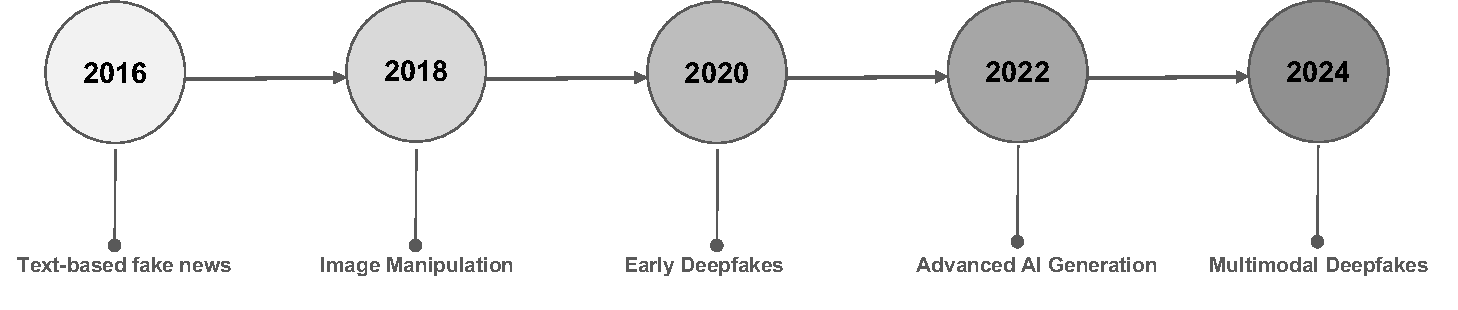
\includegraphics[width=0.8
\linewidth]{figures/figure-1.pdf}
\caption{Evolution of fake news}
\label{fig:evolution}
\end{figure}

The impact of misinformation extends well beyond public health concerns, affecting political stability and eroding public trust~\cite{mwangi2023technology}. False narratives can skew public opinion, undermine confidence in media and institutions, and even influence electoral outcomes~. As large-scale AI systems and deep-fake tools become more accessible, the ease of producing convincing fake content has intensified the urgency for robust detection methods.

In response to these challenges, our study proposes a comprehensive machine learning framework that integrates traditional learning-based methods, deep learning architectures, and large language model (LLM)-based techniques. Our approach not only targets conventional fake news but also addresses emerging threats posed by LLM-driven content manipulation. Leveraging datasets such as the WELFake collection—and augmenting them with LLM-rewritten articles generated via models like Qwen2.5-7B—we systematically evaluate and enhance the robustness and generalizability of various detection models.

The primary research question of this study is: How can advanced machine learning frameworks improve fake news detection, particularly in scenarios where sophisticated AI tools are used to manipulate content? 

Our key contributions include:
\begin{itemize}
\item Proposing an integrated framework that combines content-based semantic analysis with source reliability metrics to enhance fake news detection.
\item Conducting a comprehensive evaluation of traditional machine learning, deep learning, and transformer-based models, highlighting their strengths and limitations, particularly in detecting LLM-manipulated content.
\item Investigating model generalizability by training on both original and LLM-rewritten datasets, addressing the challenge of detecting manipulated narratives in real-world scenarios.
% \item Upon acceptance, we will publicly release our code, datasets, and model weights to ensure reproducibility and foster further research in the field.
\item For full reproducibility and to advance research in this domain, we provide open access to our codebase, datasets, and trained models through our repository at \url{https://github.com/inflaton/fake-news}.
\end{itemize}

% By presenting a holistic solution, our work aims to contribute to the ongoing efforts to maintain information integrity in an era where digital platforms and AI-driven content generation continuously evolve.

\section{Related Work}

%Due to the emergence of social media as a primary news distribution channel has fundamentally altered how information spreads. False information spreads much more quickly and reaches more people than genuine news. This premise is supported by a groundbreaking study published in Science by Vosoughi et al.~\cite{vosoughi2018spread}, which examined almost 126,000 news reports shared on Twitter. Their study revealed that incorrect material was 70\% more likely to be retweeted than content that was true, illustrating how easily misinformation spreads on social media. Automated systems are becoming more and more important in spreading false information. 

%Assessments with regard to news credibility have undergone dramatic transformations. From traditional journalistic verification to automated and sophisticated computational approaches. Sophisticated machine learning algorithms are becoming more and more important in modern approaches to news credibility assessment. A thorough review of modern detection strategies is given by Shu et al.~\cite{shu2017fakenews}, who also emphasize the trend towards integrated approaches that use several analysis techniques. Their research shows how contemporary systems use context and content elements to improve detection accuracy. A thorough analysis of fake news detecting techniques from the standpoint of data mining has identified various types of strategies. These fall into two general categories: content-based methods, which include knowledge-based and style-based approaches, and social context-based methods, which include stance-based and propagation-based strategies.

The rise of social media as a primary news source has dramatically changed how information spreads, with false information spreading faster and reaching more people than true content. A study by Vosoughi et al.~found that false news was 70\% more likely to be retweeted than accurate news, highlighting the speed of misinformation's spread~\cite{vosoughi2018spread}. Automated systems play a key role in this phenomenon.
News credibility assessments have shifted from traditional journalistic verification to advanced machine learning techniques. Shu et al.~reviewed modern fake news detection strategies, emphasizing integrated approaches that combine multiple analysis methods~\cite{shu2017fakenews}. These strategies can be divided into content-based (knowledge-based, style-based) and social context-based (stance-based, propagation-based) methods.
% \\

% \textbf{Content-based Detection Methods}
%Most early research on fake news detection mainly relied on hand-engineering relevant data that exploited linguistic features. In a ground-breaking study, Potthast et al.~\cite{potthast2018hyperpartisan} identified particular language cues which could point out problems with credibility. The study concludes that stylometric characteristics, such as word sophistication and sentence complexity patterns, are trustworthy markers in determining the legitamacy of information. The study showed that the analysis of syntactic patterns and readability indicators can reveal important information regarding the validity of content.
%Another important aspect of language evaluation is semantic analysis. According to studies, the degree of emotion in language, the clever application of technical terms, and the patterns in source attribution can all be used to distinguish between authentic and fake information. Another important predictor of content reliability has been shown to be the coherence of narrative structure.
%Linguistic analysis capabilities have advanced significantly with the use of transformer-based systems. By introducing BERT, Devlin et al.~\cite{devlin2019bert} showed previously unheard-of accuracy in identifying minor linguistic patterns suggestive of disinformation. 
\vspace{0.25\baselineskip}
\noindent \textbf{Content-based Detection Methods}
Early fake news detection research focused on hand-engineering linguistic features to assess credibility. Potthast et al.~identified language cues, such as word sophistication and sentence complexity, as reliable indicators of legitimacy~\cite{potthast2018hyperpartisan}. They found that syntactic patterns and readability could reveal content validity.
Semantic analysis also plays a key role, with emotional tone, technical terms, and source attribution helping differentiate real from fake news. Narrative coherence is another reliability predictor. Advances in linguistic analysis, particularly through transformer-based systems like BERT~\cite{devlin2019bert}, have improved accuracy in detecting subtle linguistic patterns of disinformation.

%Liu et al.~\cite{liu2019roberta} with RoBERTa and Yang et al.~\cite{yang2019xlnet} with XLNet have improved these capabilities, handling long-range dependencies in text and improving contextual understanding. The robustness of feature extraction and semantic analysis in false news detection systems has been strengthened significantly by these recent developments. Furthermore, the significance of multi-factor models in credibility evaluation was emphasized by a noteworthy study on explainable fake news identification for Polish digital media. The methodology which was used in the study integrated hybrid translation algorithms with annotator metrics and content-based approaches employing BERT and S-BERT embeddings~\cite{kozik2024explainable}. The study concluded that bias analysis and annotator demographics increased model accuracy. However, the study did also note several significant drawbacks, such as the dependence on non-expert annotators and possible errors in translated datasets. Even so, the multi-question analysis method produced extremely encouraging outcomes with a balanced accuracy of 72.1\%, indicating that integrating linguistic characteristics with annotator context can help to achieve trustworthy and accurate fake news identification ~\cite{kozik2024explainable}.

Liu et al.~with RoBERTa~\cite{liu2019roberta} 
%and Yang et al.~with XLNet~\cite{yang2019xlnet} 
enhanced fake news detection by improving long-range dependencies and contextual understanding. These advances strengthened feature extraction and semantic analysis in detection systems. A study on explainable fake news identification for Polish digital media highlighted the value of multi-factor models, combining hybrid translation algorithms, annotator metrics, and content-based approaches using BERT and S-BERT~\cite{kozik2024explainable}. The study found that bias analysis and annotator demographics improved accuracy, with a balanced accuracy of 72.1\%. However, it also noted issues with non-expert annotators and translated datasets.

%Multiple information modes are now included in modern approaches to fake news identification, which have progressed beyond basic text analysis. MVAE (Multimodal Variational Autoencoder) was created by Khattar et al.~\cite{khattar2019mvae}, which showed notable improvements in detection accuracy by integrating the study of several content types. This technique creates a more thorough detection framework by combining social signal processing, metadata analysis, and text-image consistency checking. Recent studies have extensively documented the efficacy of feature fusion approaches. Research has shown that methods that mix early and late fusion tactics are advantageous because they enable systems to take advantage of both higher-level pattern recognition and immediate feature interactions. By combining textual feature extraction, visual content analysis, and social engagement metrics, Jin et al.~\cite{jin2017microblogs} demonstrated that such multimodal approaches consistently outperform single-mode analysis, achieving accuracy improvements of up to 15\%.

Modern fake news detection has evolved to include multiple information modes beyond basic text analysis. Khattar et al.~introduced the Multimodal Variational Autoencoder (MVAE), which improved detection accuracy by integrating social signals, metadata, and text-image consistency ~\cite{khattar2019mvae}. Studies on feature fusion have shown that combining early and late fusion methods enhances both pattern recognition and immediate feature interactions. Jin et al.~demonstrated that multimodal approaches, combining textual, visual, and social features, consistently outperformed single-mode analysis, improving accuracy by up to 15\%~\cite{jin2017microblogs}.
% \\

%\newpage
% \textbf{Social Context-based Detection Methods}
%One of the most important aspects of detecting false news is the analysis of user engagement patterns. A study by Guess et al.~\cite{guess2019facebook} identified clear behavioral cues that are present during the spreading and consumption of bogus news. Their research showed that engagement depth, remark sentiment, and sharing velocity are all useful indicators of the authenticity of content. The temporal dynamics of user interactions have been particularly useful in identifying possibly fraudulent content.
%It is well known that demographic considerations have an impact on the spread of fake news. Age groupings, educational levels, and political affiliations have all been found to exhibit notable variations in sharing behaviour. These patterns provide valuable context for understanding how misinformation spreads across different demographic groupings.

%A study by Cinelli et al.~\cite{cinelli2021echo} revealed crucial insights with regards to the formation and impact of echo chambers and the significant role they play in the spread of misinformation. Varying patterns of information segregation and reinforcement were identified by their analysis of various social media sites such as Twitter and Facebook. For example, information on Twitter mainly circulates between groups with similar ideologies, where user communities seem to be more polarized than on other platforms. Facebook exhibits distinct dynamics, with the structure of groups playing a major role in reinforcing  beliefs and amplifying the spread of fake news material.
%The way these echo chambers grow is greatly influenced by platform architecture. Combining user interface components with the algorithmic architecture of content recommendation systems can result in settings that unintentionally spread false information. Del Vicario et al.~\cite{delvicario2019misinformation} showed how these structural components cause information communities to become isolated, which makes it harder for corrective information to break through preexisting belief systems and ultimately negate the effects and impact of fake news.

\vspace{0.25\baselineskip}
\noindent \textbf{Social Context-based Detection Methods}
User engagement patterns play a crucial role in detecting fake news. Guess et al.~identified key behavioral cues, such as engagement depth, sentiment, and sharing velocity, as indicators of content authenticity ~\cite{cinelli2021echo}. Temporal dynamics of user interactions are particularly useful in identifying fraudulent content.
Demographic factors, including age, education, and political affiliation, also affect the spread of fake news, influencing sharing behaviors. Cinelli et al.~~\cite{cinelli2021echo}  highlighted the role of echo chambers in spreading misinformation, finding that Twitter tends to reinforce ideological divides, while Facebook’s group structures amplify fake news. These echo chambers are shaped by platform architecture, with user interfaces and recommendation algorithms isolating information communities, making it harder for corrective content to reach users, as shown by Del Vicario et al.~\cite{delvicario2019misinformation}.
%
%\textbf{Emerging Trends and Methods}
%\\
%Since fake news frequently uses factually true elements in deceptive ways, research has repeatedly demonstrated that news content alone is insufficient for reliable detection. Research has shown that by detecting linguistic cues and social behavior patterns at the same time, integrating content and context elements produces the most accurate findings. The future of fake news detection presents both opportunities and challenges as technology continues to evolve. Research by Persily~\cite{persily2021democracy} suggests that emerging technologies, particularly in artificial intelligence and machine learning, will play an increasingly important role in combating misinformation. Advanced natural language processing techniques and improved understanding of social network dynamics offer promising avenues for future development. More recent work by Ahmed~\cite{ahmed2023kurdishfakenews} highlighted how ensemble methods and SVMs could address fake news detection in low-resourced languages. Significant improvements in performance were achieved by Ghayoomi and Mousavian~\cite{ghayoomi2022covidfake} through combining BERT models with parallel CNN classifiers. The introduction of the Longformer architecture by Beltagy et al.~\cite{beltagy2020longformer} has enhanced capabilities for processing longer documents across various NLP tasks.\\
%
% Fake news often combines true facts in deceptive ways, making content alone insufficient for reliable detection. Research shows that integrating linguistic cues with social behavior patterns yields the most accurate results. As technology advances, AI and machine learning are expected to play a larger role in combating misinformation. Persily emphasize the potential of natural language processing and social network analysis~\cite{persily2021democracy}, while Ahmed explored ensemble methods and SVMs for fake news detection in low-resourced languages~\cite{ahmed2023kurdishfakenews}. Ghayoomi and Mousavian improved performance by combining BERT with parallel CNN classifiers~\cite{ghayoomi2022covidfake}, and the Longformer architecture enhanced processing of longer documents in NLP tasks ~\cite{beltagy2020longformer}. 

% Fake news often intertwines factual information with deceptive elements, making content-based detection alone insufficient for reliable identification. Research suggests that integrating linguistic cues with social behavior patterns yields the most accurate results. 
% As artificial intelligence (AI) and machine learning continue to evolve, their role in combating misinformation is becoming increasingly significant. Persily et al.~\cite{persily2021democracy} highlight the potential of natural language processing and social network analysis, while Ahmed~\cite{ahmed2023kurdishfakenews} explores ensemble methods and support vector machines (SVMs) for fake news detection in low-resource languages. Ghayoomi and Mousavian~\cite{ghayoomi2022covidfake} enhance detection performance by combining BERT with parallel CNN classifiers, whereas Beltagy et al.~\cite{beltagy2020longformer} leverage the Longformer architecture to improve the processing of lengthy documents in natural language processing (NLP) tasks. Additionally, Ma et al.~\cite{ma2024learning} propose a multimodal framework that integrates token-level semantic consistency with frequency-domain information to effectively address challenges such as image manipulation.

As artificial intelligence (AI) and machine learning continue to evolve, their role in combating misinformation is becoming increasingly significant. Persily et al.\cite{persily2021democracy} highlight the potential of natural language processing (NLP) and social network analysis, while Ahmed\cite{ahmed2023kurdishfakenews} explores ensemble methods and support vector machines (SVMs) for fake news detection in low-resource languages. Ghayoomi and Mousavian~\cite{ghayoomi2022covidfake} enhance detection performance by combining BERT with parallel CNN classifiers, whereas Beltagy et al.\cite{beltagy2020longformer} leverage the Longformer architecture to improve the processing of lengthy documents in NLP tasks. Kumar et al.\cite{kumar2021fake} propose an XLNet fine-tuning model to predict fake news in both multi-class and binary classification scenarios, achieving results superior to existing state-of-the-art models. Bathla et al.\cite{bathla2022intelligent} propose an aspect-based deep learning approach, extracting specific aspects and their corresponding sentiment polarities from reviews to significantly enhance fake-review detection accuracy while reducing computational complexity. Recently, Ma et al.\cite{ma2024learning} introduced a multimodal framework integrating token-level semantic consistency with frequency-domain information to effectively address challenges such as image manipulation.


\section{Proposed Fake News Detection Framework}

Figure~\ref{fig:method_outline} provides an overview of our proposed framework. We aim to provide a comprehensive experimental framework for evaluating fake news detection models in the context of LLM-rewritten content, by systemically comparing the performance across model categories under normal conditions, followed by manipulated input conditions. The process begins with the \emph{text dataset} and proceeds to a comprehensive \emph{data pre-processing} phase—which includes cleaning, tokenization, vectorization, and other preparatory steps—before advancing to \emph{model construction}. In this phase, three categories of models are explored:
\begin{enumerate}
    \item \textbf{Traditional Learning-Based Models} (e.g., Random Forest, SVM) with traditional feature engineering techniques (e.g., Count Vectorizer, stemming),
    \item \textbf{Deep Learning-Based Models} (e.g., CNN, RNN, LSTM) employing embedding approaches (e.g., Word2Vec, GloVe), and
    \item \textbf{Transformer-based models} (e.g., BERT, RoBERTa, DistilBERT).
\end{enumerate}

After model construction, \emph{model training} is performed with hyperparameter tuning. Finally, \emph{performance evaluation} is conducted using metrics such as accuracy, precision, recall, and F1-score to assess the effectiveness of each model.

\begin{figure}[!htbp]
    \centering
    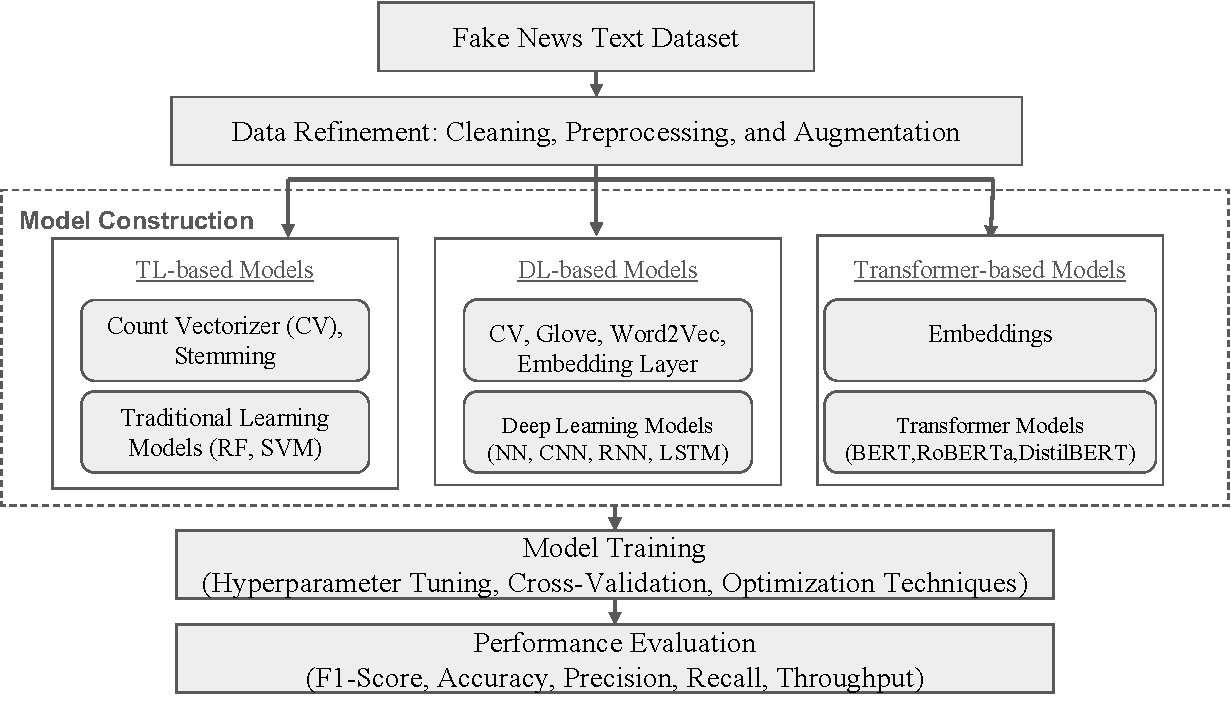
\includegraphics[width=0.9\textwidth]{figures/figure-2.pdf}
    \caption{Outline of the proposed method.}
    \label{fig:method_outline}
\end{figure}

\subsection{Datasets}

For training and validating our models, we utilized the WELFake dataset for fake news detection in text data~\cite{welfake2021}, a comprehensive collection of 72,134 news articles curated specifically for fake news classification tasks.

\noindent \textbf{Data Cleaning}
The data cleaning process begins with feature selection, focusing on the \texttt{title}, \texttt{text}, and \texttt{label} columns to retain only relevant information. Duplicate rows are removed to maintain data integrity and avoid redundancy. Outliers are detected and eliminated based on a 3-standard deviation (3~SD) criterion applied to the lengths of the \texttt{title} and \texttt{text} fields, ensuring consistent data quality. The \texttt{title} and \texttt{text} columns are then concatenated to form a new \texttt{full\_content} column, with missing values imputed as empty strings. Subsequently, the original \texttt{title} and \texttt{text} columns are dropped to streamline the dataset. Finally, rows with empty \texttt{full\_content} fields, those containing fewer than 30 words or more than 2000 words, and non-Enlish articles are removed.%and articles written in languages other than English are removed.

\noindent \textbf{Data Preprocessing}
To further standardize and normalize the text data, we create a new column, \texttt{processed\_full\_content}, by applying a custom text processing function to the \texttt{full\_content} column. This function converts the text to lowercase, tokenizes it, removes punctuation, filters out common stopwords while retaining key negation words, and applies stemming using the Porter Stemmer. These preprocessing steps ensure that the text is cleaned and normalized, making it suitable for subsequent model training and evaluation.
After this, we obtained a refined dataset containing 60,491 entries with three columns: \texttt{label}, \texttt{full\_content}, and \texttt{processed\_full\_content}. The dataset consists of 34,030 true news articles (\texttt{label} = 0) and 26,461 fake news articles (\texttt{label} = 1). We refer to this as the \textbf{original} dataset.

\noindent \textbf{Dataset Expansion}
% To evaluate the generalizability of our models, we employed the Qwen2.5-7B model to rewrite all \texttt{full\_content} entries. The rewriting process was guided by carefully designed prompts that ensured clarity, readability, and engagement while preserving all original details and factual accuracy. Specifically, we used the following prompt template:
To assess the generalizability of our models, we utilized the Qwen2.5-7B model to rewrite all \texttt{full\_content} entries. Qwen2.5-7B was chosen for its optimal balance between computational efficiency and linguistic capability. The rewriting process was guided by carefully crafted prompts, as illustrated in the following template:
\begin{minted}[fontsize=\footnotesize, breaklines]{text}
Rewrite the following text to improve clarity, readability, and engagement while maintaining all original details and factual accuracy. Use concise, natural phrasing, and enhance flow without omitting any information. Ensure that the structure is logical, sentences are varied in length, and transitions are smooth. The tone should remain neutral and professional, suitable for a news article or formal report. Avoid redundancy while keeping all key details intact.
{input}
\end{minted}

% \noindent
In this template, the \texttt{\{input\}} placeholder is replaced with the \texttt{full\_content} of each article before it is submitted to the Qwen2.5-7B model.

The rewritten content generated by the Qwen2.5-7B model was subsequently processed using the same text preprocessing steps applied to the original dataset, resulting in the \texttt{processed\_full\_content} column. This newly generated dataset is referred to as the \textbf{LLM-rewritten} dataset. By combining both the original and LLM-rewritten datasets, we constructed a third dataset, denoted as the \textbf{combined} dataset.

% All datasets were subsequently split into a training set (90\%) and a test set (10\%) for model evaluation.

\subsection{Model Construction}

% \vspace{0.5\baselineskip}
\noindent \textbf{Traditional Learning-Based Models}
% \vspace{0.5\baselineskip}
% 
To establish a baseline for fake news detection, we employed two widely recognized machine learning algorithms, e.g., Random Forest (RF) and Support Vector Machines (SVM), along with Term Frequency Inverse Document Frequency Vectorizer (TF-IDF) and stemming for feature extraction. This blend of classic feature engineering techniques and traditional algorithms serves as a valuable benchmark for evaluating more advanced approaches.


\vspace{0.25\baselineskip}
\noindent \textbf{Deep Learning-Based Models}
% \vspace{0.5\baselineskip}
% 
In contrast to traditional approaches, deep learning-based methods utilize learned or pre-trained word embeddings rather than manually engineered features. GloVe and Word2Vec are popular examples of pre-trained embeddings, while an Embedding layer allows for trainable embeddings. Due to the strong performance of deep learning in text classification tasks, we included several neural network architectures—specifically, feed-forward neural networks (NN), convolutional neural networks (CNN), recurrent neural networks (RNN), and long short-term memory networks (LSTM).


\vspace{0.25\baselineskip}
\noindent \textbf{Transformer-Based Models}
% \vspace{0.5\baselineskip}
% 
Large Language Models (LLMs), based on the Transformer architecture, are at the forefront of natural language understanding. These models excel at capturing contextual and semantic nuances in text by employing attention mechanisms that process entire sequences of words. This enables them to capture long-range dependencies and bidirectional relationships. Notably, BERT utilizes self-attention, achieving exceptional performance across various NLP tasks. We have selected BERT, DistilBERT, and RoBERTa for our experiments due to their proven effectiveness in text classification.

% \vspace{0.5\baselineskip}
% \noindent
% Overall, this model construction phase examines traditional, deep learning, and LLM-based methods, providing a comprehensive understanding of their strengths and weaknesses in addressing fake news detection.

\subsection{Model Training}

Once the models have been constructed, the next phase involves training them on the datasets. To ensure robust performance and mitigate overfitting, we employ several strategies during training:

\vspace{0.25\baselineskip}
\noindent \textbf{Hyperparameter Tuning:} Extensive hyperparameter optimization is performed using techniques such as grid search and random search. This process fine-tunes key parameters—including learning rates, regularization strengths, and network architectures—to identify the optimal configuration for each model.
    % (e.g., number of layers and neurons)
    
\vspace{0.25\baselineskip}
\noindent  \textbf{Cross-Validation:} For traditional learning-based models, we employ 5-fold cross-validation to evaluate generalizability and robustness across different subsets of the dataset. Once the optimal hyperparameters are identified, a final training run is conducted on 90\% of the dataset to further enhance performance.
    
\vspace{0.25\baselineskip}
\noindent  \textbf{Optimization Techniques:} Advanced optimization algorithms, such as Adam and stochastic gradient descent (SGD), are utilized to efficiently minimize the loss function, thereby accelerating the convergence of deep learning models and improving their training stability.
    
    % \item \textbf{Resource Management:} Given the computational demands of deep learning and transformer-based approaches, training is performed on an NVIDIA RTX A6000 Ada Generation GPU, featuring 48\,GB of GDDR6 ECC memory, 18,176 CUDA cores, and 568 Tensor cores. 
    % This high-performance hardware significantly accelerates training and enables the handling of large datasets and complex models. This is referred to as RTX A6000 throughout this paper.

\vspace{0.25\baselineskip}
\noindent \textbf{Resource Management:} Given the computational demands of deep learning and transformer-based approaches, training is performed on an NVIDIA RTX A6000 Ada GPU (48\,GB GDDR6 ECC memory, 18,176 CUDA cores, 568 Tensor cores), referred to as RTX A6000 throughout this paper.

\subsection{Evaluation Metrics}

We assess model performance using four key metrics: \textbf{accuracy}, \textbf{precision}, \textbf{recall}, and \textbf{F1-score}, ensuring a comprehensive evaluation of classification effectiveness. To measure computational efficiency, we also evaluate \textbf{throughput}, defined as the number of samples processed per second:

\begin{equation}
    \text{Throughput} = \frac{\text{Total samples processed}}{\text{Total processing time (s)}}
\end{equation}

Higher throughput enables faster processing, essential for real-time or large-scale applications. All experiments were consistently run on the RTX A6000.

\section{Results and Discussion}

\subsection{Performance Comparative Analysis Using Original Data}
To assess model effectiveness in fake news detection, we trained and tested various machine learning models using the original WELFake dataset. Table~\ref{tab:model_performance_metrics} summarizes our evaluation results.
% , comparing \textbf{accuracy}, \textbf{precision}, \textbf{recall}, \textbf{F1-score}, and \textbf{throughput} across different models. 
% Additionally, we report \textbf{throughput}, measured in samples processed per second using an Nvidia GeForce RTX 4090 Laptop GPU, to evaluate computational efficiency.

\begin{table}[!htbp]
  \centering
  \caption{Performance Comparison of Machine Learning Models for Fake News Detection. All models are trained and evaluated using the original WELFake train/test data. Highest performance metrics are highlighted in bold.}
  \label{tab:model_performance_metrics}
  \begin{tabular}{lccccc}
    \toprule
    \textbf{Model} & \textbf{Accuracy} & \textbf{Precision} & \textbf{Recall} & \textbf{F1-Score} & \textbf{Throughput} \\
    \midrule
    RF & 0.9494 & 0.9415 & 0.9430 & 0.9422 & \textbf{1242} \\
    SVM & 0.9698 & 0.9642 & 0.9668 & 0.9655 & 1175 \\
    Simple Neural Network & 0.9646 & 0.9645 & 0.9543 & 0.9594 & 805 \\
    CNN & 0.9775 & 0.9776 & 0.9709 & 0.9742 & 836 \\
    RNN & 0.9428 & 0.9492 & 0.9184 & 0.9336 & 628 \\
    LSTM & 0.9779 & 0.9805 & 0.9686 & 0.9745 & 617 \\
    BERT & 0.9945 & 0.9921 & \textbf{0.9955} & 0.9938 & 197 \\
    RoBERTa & 0.9931 & 0.9917 & 0.9924 & 0.9921 & 139 \\
    DistilBERT & \textbf{0.9949} & \textbf{0.9928} & \textbf{0.9955} & \textbf{0.9942} & 201 \\
    \bottomrule
  \end{tabular}
\end{table}

Our experimental results reveal several key findings. Among all models, transformer-based architectures (BERT, RoBERTa, and DistilBERT) consistently outperform traditional machine learning and neural network approaches in classification metrics. \textbf{DistilBERT} achieves the highest performance across all classification metrics, with an accuracy of \textbf{99.49\%}, precision of \textbf{99.28\%}, recall of \textbf{99.55\%}, and F1-score of \textbf{99.42\%}. This superior performance can be attributed to the model's ability to capture complex contextual relationships in text through its pre-trained language understanding capabilities.

However, the computational efficiency analysis presents an interesting trade-off. While transformer models excel in accuracy, they exhibit significantly lower throughput rates. Traditional machine learning models—particularly \textbf{RF and SVM}—demonstrate substantially higher processing speeds (\textbf{1242} and \textbf{1175} samples per second, respectively) compared to transformer models (201 samples/s for DistilBERT, 197 samples/s for BERT, and 139 samples/s for RoBERTa). This performance-efficiency trade-off becomes crucial when considering real-world deployment scenarios where both accuracy and speed are important.

Among the neural network architectures, LSTM shows promising results with an accuracy of 97.79\% and an F1-score of 97.45\%, while maintaining moderate throughput (617 samples/s). The CNN model also performs well, achieving 97.75\% accuracy with better throughput (836 samples/s) compared to recurrent architectures. In contrast, the Simple Neural Network and RNN exhibit relatively lower performance metrics but maintain competitive processing speeds.

These findings suggest that the choice of model for fake news detection should be guided by the specific requirements of the application context. For high-stakes applications where accuracy is paramount, transformer-based models—particularly \textbf{DistilBERT}—would be the optimal choice. However, for real-time applications where processing speed is critical, traditional machine learning models like \textbf{RF} might be more suitable, as they offer a better balance between accuracy and computational efficiency.

\subsection{Model Generalizability and LLM Impact Analysis}
\label{subsec:llm_impact}

While our initial performance analysis using the original WELFake dataset showed promising results, we conducted additional experiments to evaluate model generalizability and assess the impact of LLM-rewritten content on detection accuracy. Figure~\ref{fig:model_generalization} presents a comparative analysis of both F1 Score and Throughput on the original and LLM-rewritten test sets under two training scenarios.

\begin{figure}[!htbp]
    \centering
    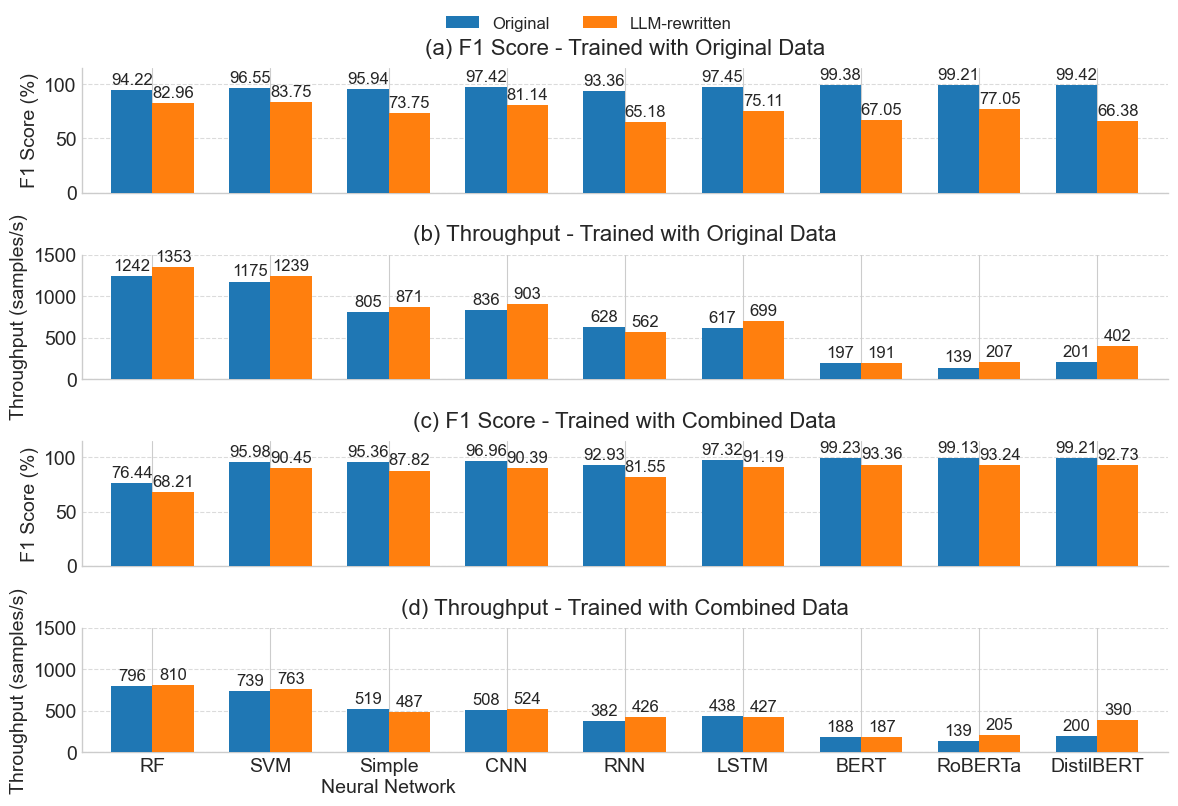
\includegraphics[width=.9\textwidth]{figures/original_vs_rewritten.png}
    \caption{Comparative analysis of F1 Score and Throughput for various models evaluated on \emph{original} vs. \emph{LLM-rewritten} test articles. 
    Subplots (a) and (b) show models trained only on the original dataset, while subplots (c) and (d) show models trained on the combined dataset.}
    \label{fig:model_generalization}
\end{figure}

When trained solely on the original dataset, all models exhibit excellent performance on the original test set, with transformer-based models achieving F1-scores above 99\%. However, performance degrades considerably when evaluated on the LLM-rewritten test set. The drop is particularly pronounced for transformer models, with DistilBERT’s F1-score falling from 99.42\% to 66.38\%—a reduction of over 33 percentage points. Similar substantial declines are observed for BERT (99.38\% to 67.05\%) and RoBERTa (99.21\% to 77.05\%). By contrast, traditional machine learning models display relatively better resilience, with RF and SVM showing smaller performance gaps (11.26\% and 12.80\%, respectively).

To address this generalizability challenge, we trained models on the combined dataset, which contains both original and LLM-rewritten articles. This approach significantly improves performance on the LLM-rewritten content across all models, albeit with a slight trade-off in performance on the original articles. 

Notably, the gap between performance on the original and LLM-rewritten content narrows substantially, and transformer models achieve more consistent results. For example, DistilBERT attains F1-scores of 99.21\% and 92.73\% on original and LLM-rewritten articles, respectively, reducing the performance gap to 6.48\%.
From subplots (b) and (d) of Figure~\ref{fig:model_generalization}) we observe a consistent drop in throughput for most models when trained on the combined dataset compared to the original dataset, likely reflecting the increased complexity of handling both original and LLM-rewritten articles. For instance, the throughput of SVM decreases from 1,175 samples/s when trained on the original dataset to 739 samples/s when trained on the combined dataset. Similarly, DistilBERT's throughput drops from 402 samples/s to 390 samples/s, indicating a slight computational overhead when incorporating LLM-rewritten content. Despite these reductions, the overall throughput ranking remains consistent, with RF (810 samples/s) and SVM (763 samples/s) achieving the highest inference speed, while transformer-based models such as BERT (187 samples/s) and RoBERTa (205 samples/s) continue to exhibit significantly lower throughput due to their computational complexity. Notably, DistilBERT strikes a balance between robust F1 performance and relatively faster inference speed, making it an attractive option for resource-constrained scenarios where both accuracy and efficiency are critical.

These findings underscore a critical challenge in modern fake news detection: LLM-rewritten content can substantially compromise the effectiveness of models trained on traditional datasets. While combining original and LLM-rewritten samples in training yields notable improvements, the residual performance gap indicates that further research is needed to fully counter LLM-driven content manipulation in fake news detection.

\section{Conclusion}
\label{sec:conclusion}

In this work, we introduced a comprehensive framework for fake news detection that spans traditional machine learning, deep learning, and transformer-based approaches. Our methodology was designed to address not only the challenges posed by naturally occurring news content but also those introduced by advanced text manipulation through LLM-based rewriting. Our experimental results highlight several key insights:
\begin{itemize}
\item Transformer-based models, particularly DistilBERT, achieve outstanding classification metrics on the original dataset. However, their performance degrades significantly when evaluated on LLM-rewritten content, indicating a vulnerability in handling sophisticated text manipulations.
\item Traditional models, while slightly less accurate overall, demonstrated more resilience to content alterations, suggesting that a balance between high accuracy and robust generalizability is crucial.
\item Incorporating both original and LLM-rewritten samples in the training process markedly improved model performance on manipulated content, though a performance gap still persists.
\end{itemize}

In this work, we provide the community with a public dataset of LLM-rewritten fake/real news articles, which can serve as a valuable benchmark for future adversarial robustness studies. These findings underscore the necessity for ongoing research into more robust detection strategies that can adapt to the evolving landscape of content generation. Future work should focus on:
\begin{enumerate}
% \item Enhancing model architectures to better capture subtle cues in manipulated text,
\item Expanding research across diverse datasets and leveraging multiple LLMs for rewritten content to enhance generalizability,
% Different LLMs may introduce distinct linguistic styles, structural variations, or subtle biases, potentially affecting detection performance. A comparative analysis across models would provide deeper insights into how various text manipulations influence generalizability.
\item Integrating adaptive learning techniques for real-time updates with emerging data, and
\item Conducting further investigations into the impact of fully LLM-generated content on detection efficacy.
\end{enumerate}

Overall, our study demonstrates that while current detection systems are effective on traditional datasets, they require continual refinement to remain robust against the sophisticated techniques enabled by modern language models. Addressing these challenges is vital for developing reliable, real-world fake news detection systems.

% \iffalse
\section*{Acknowledgment}

The authors express their sincere appreciation to the following SMU students for their keen interest and valuable contributions to the code and report development of this research: LEE Ryan, Sakthivel GANAPATHY, See Jae FOO, Abhay BAGDAWALA, Shaun ZHOU, Gabriel CHUA, Arthur CHENG, 
Cristie SIM,
Pei Shyan LIM, 
Seah WANG,
Jin Sheng TEOH,
and Hai Xiang ONG
.
% \fi

% ---- Bibliography ----
%
\bibliographystyle{splncs04}
\bibliography{mybibliography}
%
\end{document}
